This thesis set out to create a parametric L-system capable of representing complex plant-like structures. And to use the L-system to procedurally generate plant-life with all of the relavant information necessary for physical simulation. This chapter will test several features of the parametric L-system, such as how to varying branch width and branching angles, and how to produce different effects on the resulting plant models. Furthermore, this chapter provides several different examples that will test the physical simulation by varying parameters in the L-system. All of the tests are run on the same interpreter and physics simulation, with the acceleration due to gravity being kept at a constant value of $9.8m/s^2$. 

The parametric L-system in \ref{L-system params} below, contains several variables that can be manipulated to change the visual properties of the rendered tree. The next few examples will illustrate how the use of these parameters can effect the look of the plant and how the plants reacts differently when simulated. The table shows three sets of default values that will be applied to the L-system in each example. One or two of these parameters will be changed and a screenshot showing its effect on the plants structure or how it reacts in the simulation will be shown.

Each variable in the table below represents a particular feature that can be manipulated. These features have the the following meanings: 


\begin{itemize}[noitemsep]
	\item n - The number of generations to rewrite
	\item a1 - The angle of the first pitch rotation in production rule 1
	\item a2 - The angle of the second pitch rotation in production rule 1
	\item a3 - The angle of both roll rotations in production rule 1
	\item dl - The proportion to increase the branch length each generation
	\item dr - The proportion to increase the branch width each generation
	\item scstart - The starting spring constant 
	\item scmod - The proportion to increase the spring constant each generation
\end{itemize}

\vspace{10mm}
\hrule
\begin{singlespace}
\begin{equation}
\begin{aligned}
	&\textrm{\#object F BRANCH;}\\
	&\textrm{\#w : !(1.4)F(2.0, scstart)/(45)A(scstart);}\\
	&\textrm{\#p1 : A(sc) : * : !(dr)F(2, sc)[\&(a3)F(2, sc)A(sc)]/(a1)[\&(a3)F(2, sc)A(sc)]/(a2)[\&(a3)F(2, sc)A(sc)];}\\
	&\textrm{\#p2 : F(l, sc) : * : F(l*dl, sc*scmod);}\\
	&\textrm{\#p3 : !(w) : * : !(w*dr);}
\end{aligned}
\end{equation}
\end{singlespace}

\begin{table}[h!]
\centering
\begin{tabular}{ | c | c | c | c | c | c | c | c | c | }
\hline
	Variation Name & n & a1 & a2 & a3 & dl & dr & scstart & scmod\\  
\hline
\hline
	L-system 1  & 6 & 112.5 & 157.5 & 22.5 & 1.1 & 1.4 & 200 & 1.0 \\
\hline
	L-system 2  & 6 & 137.5 & 137.5 & 18.95 & 1.1 & 1.2 & 200 & 1.0 \\
\hline
	L-system 3  & 7 & 112.5 & 157.5 & 22.5 & 1.1 & 1.4 & 200 & 1.0 \\
\hline
\end{tabular}
\caption{Table of turtle graphics instructions symbols and their meaning to the interpreter}
\label{L-system params}
\end{table}
\FloatBarrier
\hrule

\vspace{10mm} 

\noindent
In the example in figure \ref{example thickness}, the value `dr', manipulates how thick each branch is. It does this during the rewriting process. Every time the width module `!' is encountered, it is rewritten with the current radius multiplied by the value of `dr', which increases the radius exponentially. This relationship can be expressed as $r_{i+1} = r_i \times dr$, where $r_i$ is the current branch radius and $r_{i+1}$ is the radius of the branch in the next generation. This gives a tree that gets thicker exponentially as the branch moves closer to the base of the tree. This can be shown in the graphs in figure \ref{graph thickness} below. For a tree that gets thicker linearly, the relationship can be changed and expressed as $r_{i+1} = r_i + dr$. This would result in a tree that gets thicker much more progressively.

Although this example is not a physical simulation, it could be simulated. Due to the larger width of the branches near the base of the tree, they would have a higher mass and therefore have more inertia, making them more resistant to changes in velocity.

\begin{figure}[htbp]
	{\centering
		\vspace{7px}
		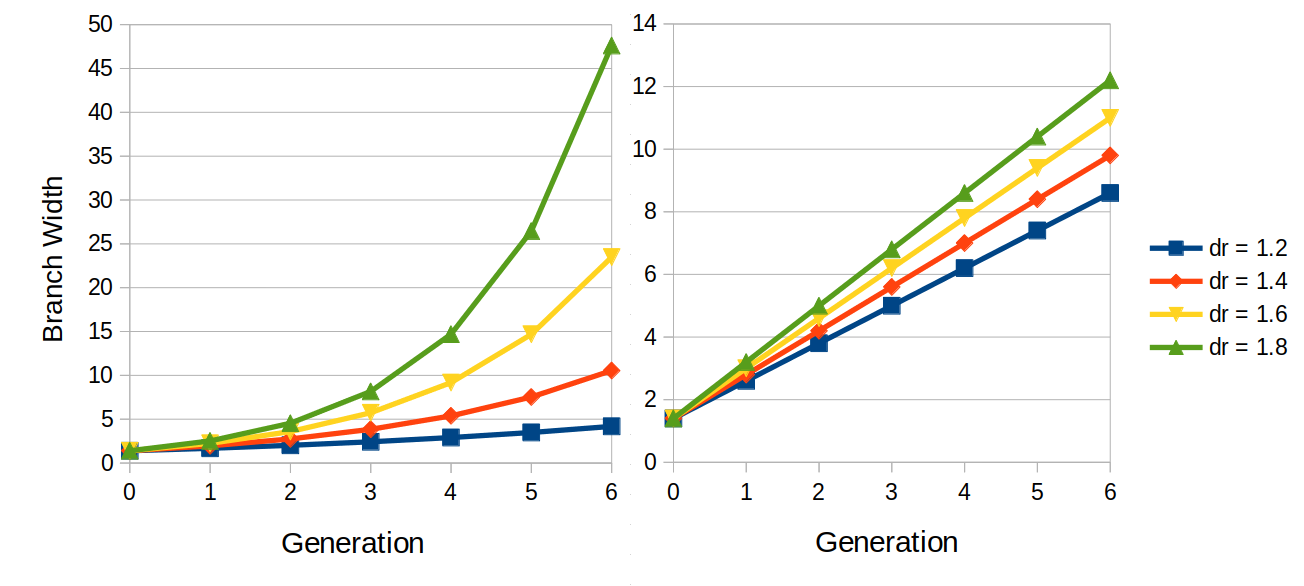
\includegraphics[scale=0.35]{Diagrams/branchWidthIncrease.png}
		\caption{Graph showing an exponential and linear relationship between the branch width and the generation when increasing the value of `dr'.} \label{graph thickness}
	}
\end{figure}
\FloatBarrier

\begin{figure}[htbp]
	{\centering
		\vspace{7px}
		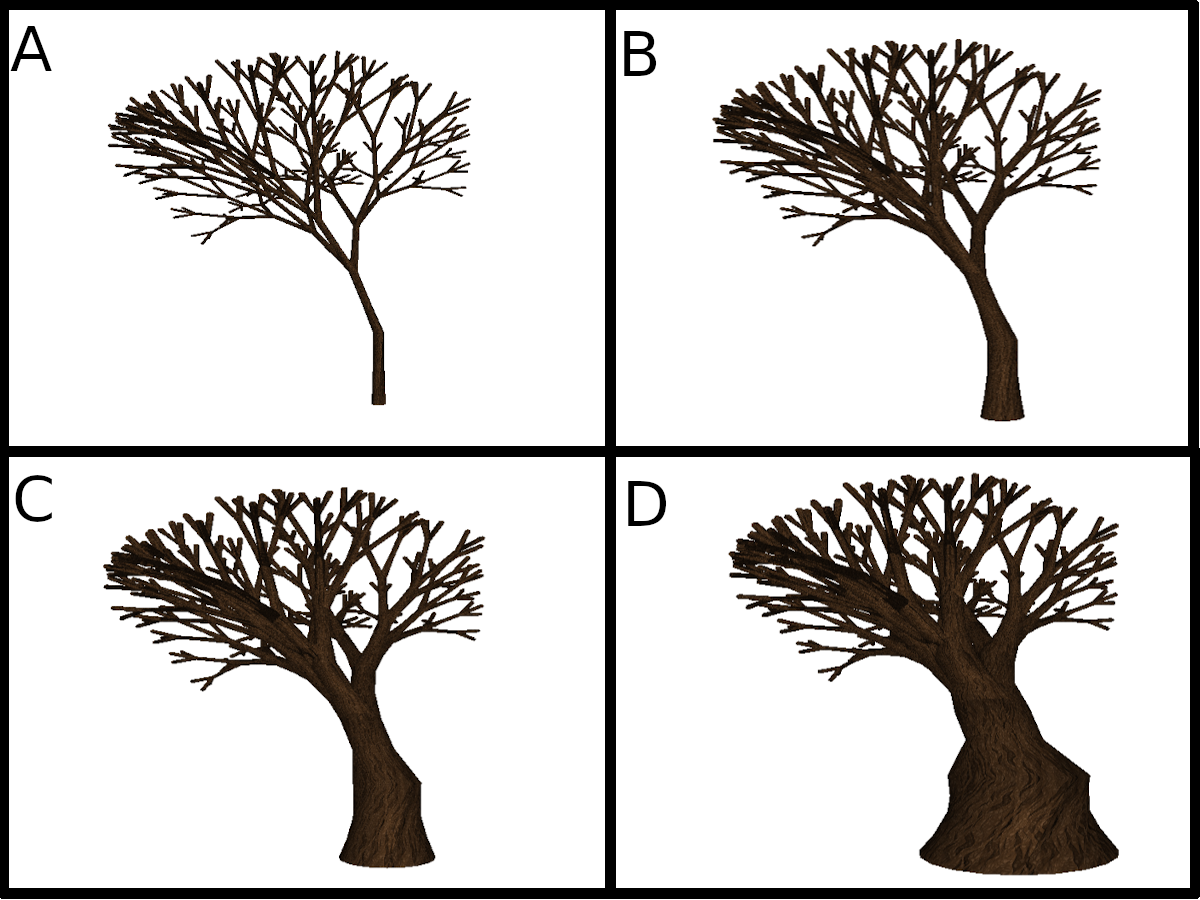
\includegraphics[scale=0.30]{Diagrams/TernaryBranching3_vr.png} 
		\caption{Examples of L-system 1 changing the `dr' variable which modifies the thickness of the base of the tree.} \label{example thickness}
	}
\end{figure}
\FloatBarrier

\noindent
In figure \ref{example angle} below shows that the result of changing the roll rotations' angle for some of the branches gives the tree a very different shape. In this case, increasing the angle of the branches' roll rotation from 15$^\circ$ to 30$^\circ$ can create a branch that curls slightly. Increasing this angle causes a more dramatic result. Furthermore, the angles of rotations can be randomised using the random range feature of the L-system to create a tree with more erratic branches. Manipulating the angles of rotations is a very powerful tool to allow very drastic changes to the look or behavior of a plant without changing its structure. 

\begin{figure}[htbp]
	{\centering
		\vspace{7px}
		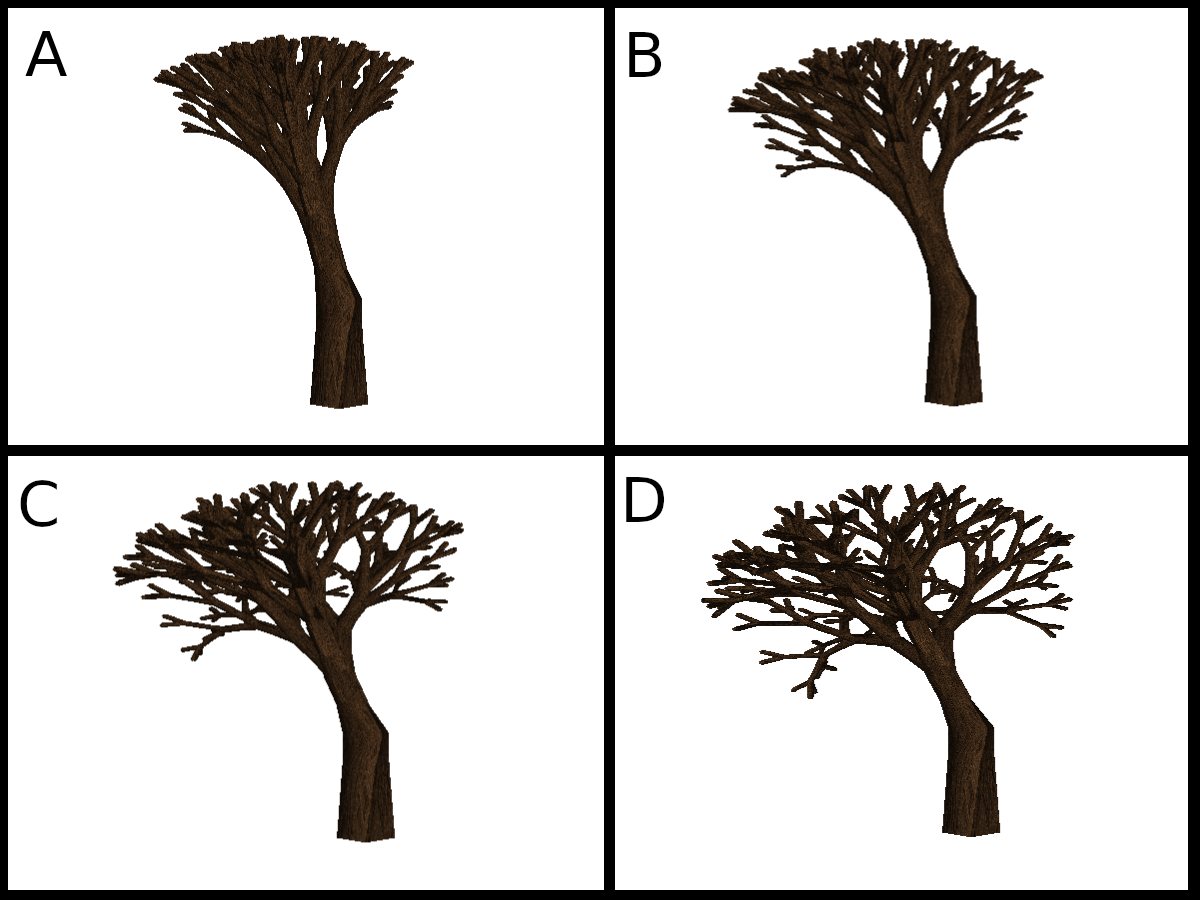
\includegraphics[scale=0.30]{Diagrams/TernaryBranching2_angle_example.png}
		\caption{Examples of L-system 2 changing the `a3' variable modifying the roll angle of certain branches.} \label{example angle}
	}
\end{figure}
\FloatBarrier

The previous examples have tested the capabilities of the parametric L-system without having the resulting structures simulated. One of the advantages of having the simulator and interpreter separate to the L-system rewriter is that the simulator and interpreter choose to ignore specific parameters. For instance, the physical properties of a plant may be provided by the L-system, but the simulator can be turned off, resulting in a static plant that is less resource-intensive to render as it is not continuously updated. The next examples show that changing the physical properties of the plant can change how it responds when the simulator is turned on. Each screenshot is taken after five seconds of the simulator running; this allows the branches' movement to settle into their resting position.

In figure \ref{constant spring} below, the spring constant `scstart' of the is changed from 200 down to 50.  However, the spring constant modifier `scmod' is 1.0. The spring constant for each branch is rewritten with the current spring constant multiplied by the spring constant modifier. This gives the relationship similar to how the width is calculated $sc_{i+1} = sc_i * scmod$. If the `scmod' value is 1.0, the spring constant will be a uniform value independant of how many generations there are. Leaving the spring constant the same throughout the tree assumes that thick branches at the base of the tree are as bendy as thin branches at the top of the tree. This is not accurate and will result in large branches bending unrealistically, particularly under extreme forces. Although this kind of behaviour would not be realistic, it highlights the flexibility of the system, such that if someone changes the physical properties within the L-system it will have a direct affect on the resulting model and simulation.

\begin{figure}[htbp]
	{\centering
		\vspace{7px}
		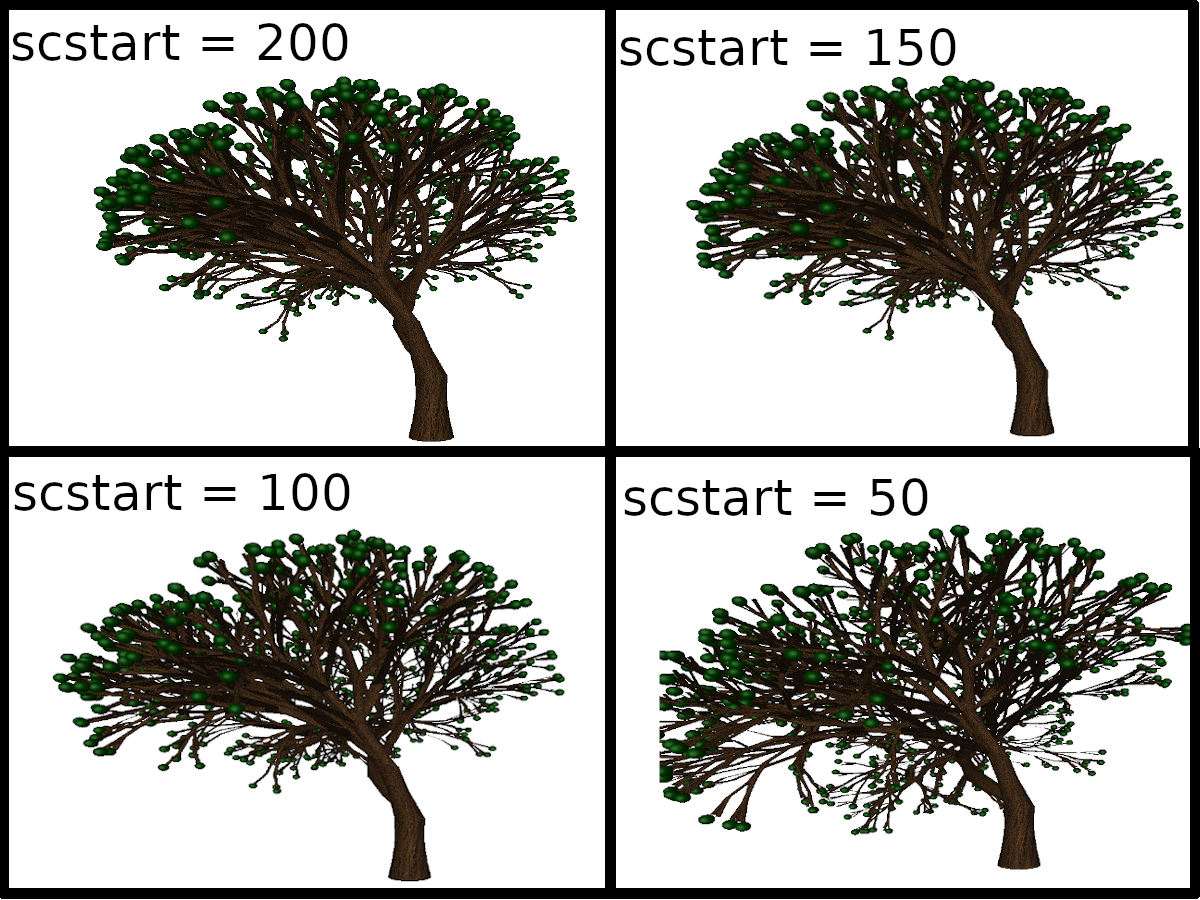
\includegraphics[scale=0.30]{Diagrams/TernaryBranching3_constantSC.png}
		\caption{Examples of L-system 1 when uniformly changing the `scstart' for all branches and leaving `scmod = 1.0'.}\label{constant spring}
	}
\end{figure}
\FloatBarrier

\noindent
In order to create a more realistic simulation where thinner branches bend more than thicker ones, the initial spring constant can be set to 30. The `scmod' value can be increased, resulting in the branches closer to the base being exponentially stiffer. Therefore, branches closer to the top are week and susceptible to smaller forces moving them around. As seen in figure \ref{increasing scmod} below, when the modifier is very high, the larger branches hardly bend at all, whereas, with a lower modifier, the larger branches visibly bend. The graphs in figure \ref{spring constant graphs} show the different ways spring constant and spring constant modifier can be changed to produce different types of branch strengths within the L-system rewriter.

\begin{figure}[htbp]
	{\centering
		\vspace{7px}
		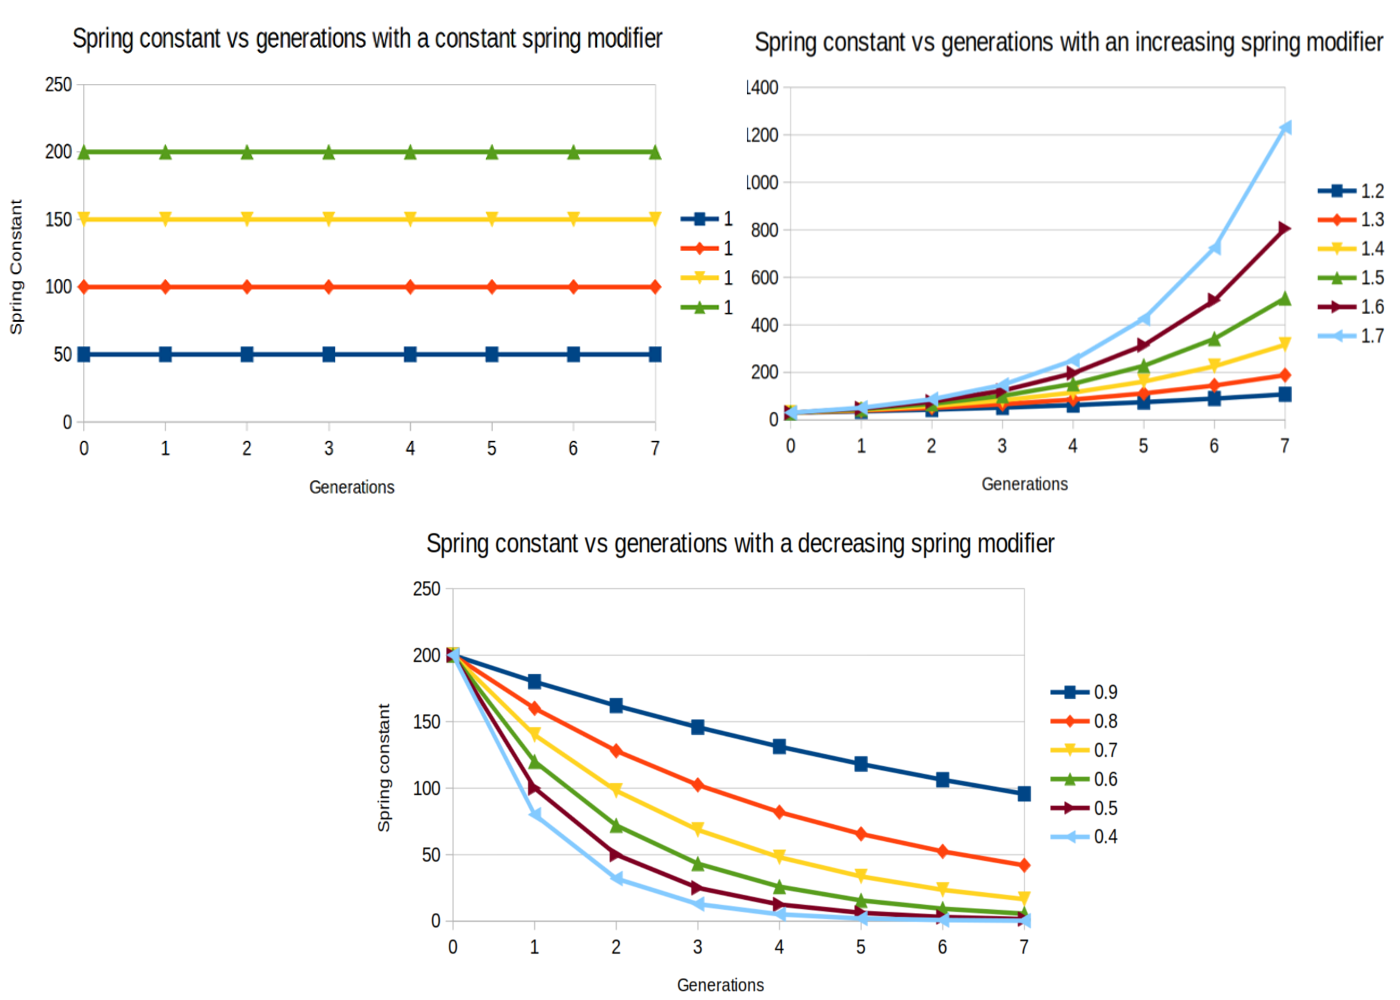
\includegraphics[scale=0.30]{Diagrams/springconstantgraphs.png}
		\caption{Graphs showing the distribution of spring constants dependency on the spring modifier and number of generations.}\label{spring constant graphs}
	}
\end{figure}
\FloatBarrier

\begin{figure}[htbp]
	{\centering
		\vspace{7px}
		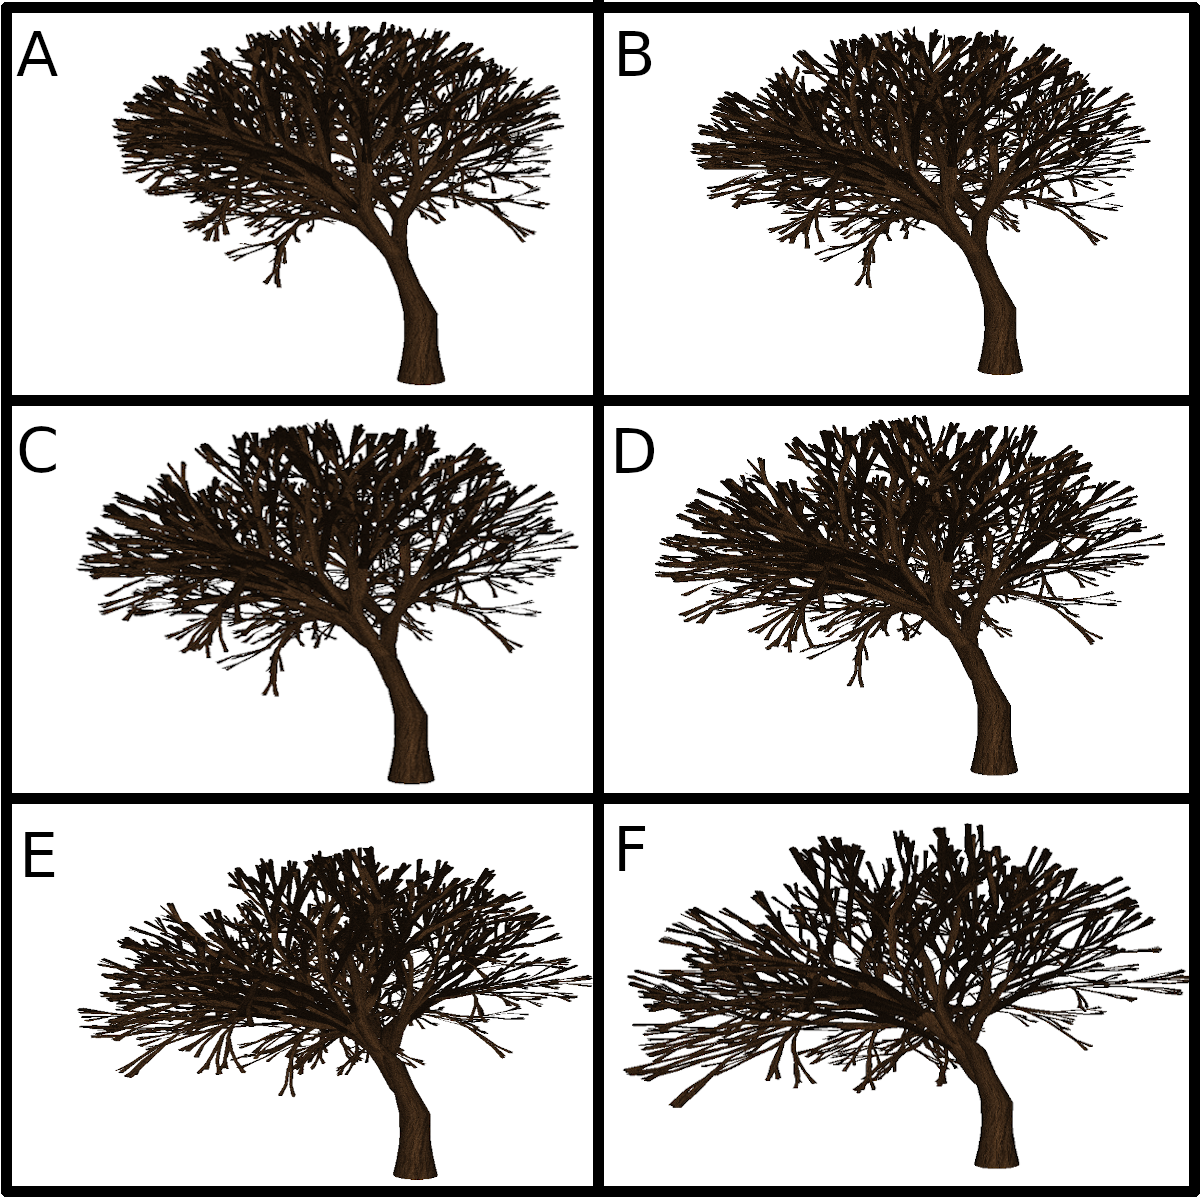
\includegraphics[scale=0.30]{Diagrams/TernaryBranching3_scmod.png}
		\caption{Examples of L-system 3 with gravity applied when changing the spring constant modifier `scmod', when the starting spring constant is set to 30 `scstart = 30'.}\label{increasing scmod}
	}
\end{figure}
\FloatBarrier

\noindent
The L-system \ref{2d L-system physics} below creates the 2D fractal tree that has rendered in three dimensions. It is a 2D tree as it only consists of left and right yaw rotations signified with the `+ and -' symbols without any pitch or roll rotations. In this tree, the rotation `r' is defined as 20$^{\circ}$, the distance `d' is 0.4, and the width `w' is 0.5. The spring constant of the branches is kept at a constant 30.0. This means that all the branches are equally prone to bending. 

\begin{singlespace}
\begin{equation} \label{2d L-system physics}
\begin{aligned}
	&\textrm{\#n = 6;} \\
	&\textrm{\#define r 20; \#define d 0.4; \#define w 0.5;}\\
	&\textrm{\#w : !(w)Z;}\\
	&\textrm{\#p1 : Z : * : F(d, 30.0)[-(r)Z]F(d, 30.0)[+(r)Z]-(r)Z;}\\
	&\textrm{\#p2 : F(s, x) : * : F(s, x)F(s, x);}
\end{aligned}
\end{equation}
\end{singlespace}

\begin{figure}[htbp]
	{\centering
		\vspace{7px}
		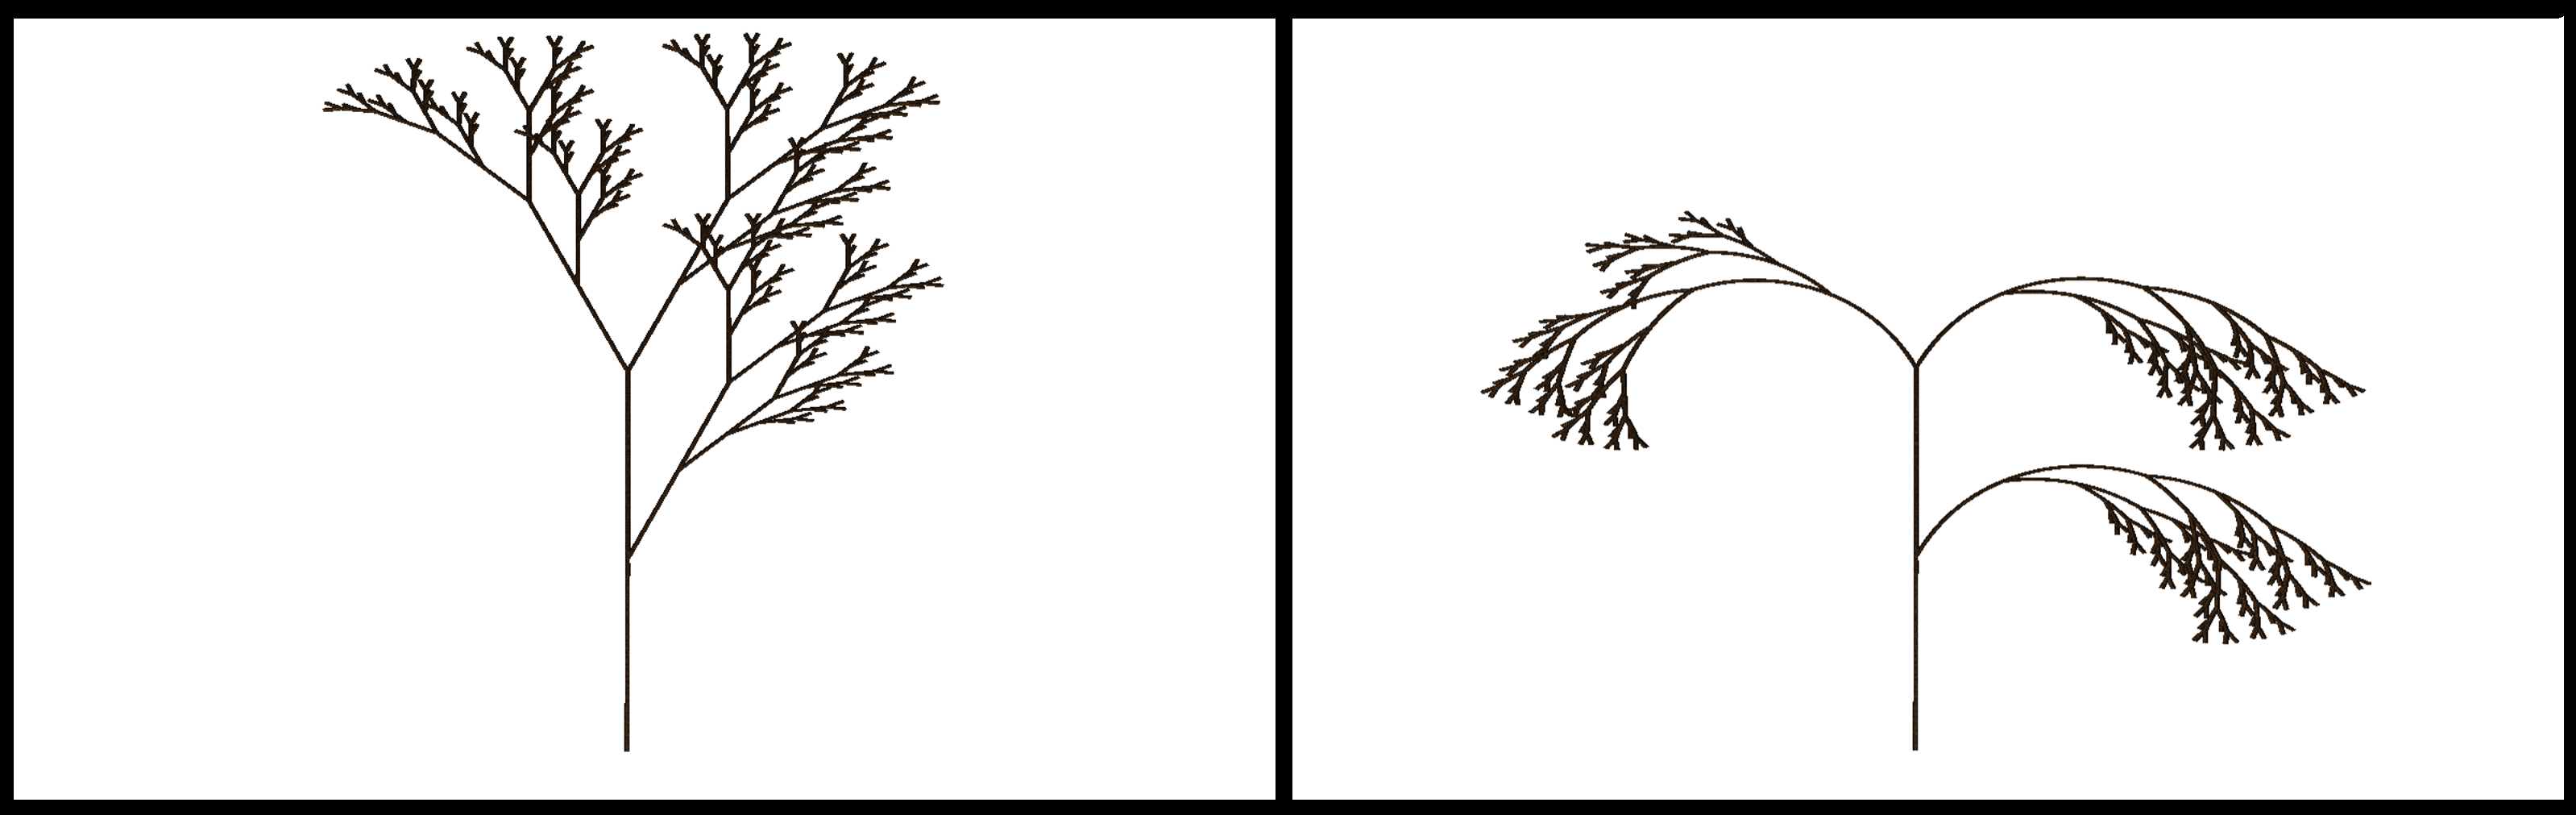
\includegraphics[scale=0.1]{Diagrams/gravityExamples1.png}
		\label{3DAxisFigure} \label{Gravity applied to generated models 1}
		\caption{Examples simulating gravity on a 2D model}
	}
\end{figure}
\FloatBarrier

\noindent
Writing the L-system for plants that are symetrical is the most straightforward. For instance the tree in figure \ref{Gravity applied to generated models 2} below has a similar structure to a pine tree. Which is a single center branch that has four branches in different directions at several points off the center branch. Although the structure of the plant is very different to the previously mentioned L-systems, providing the parameters for simulation is very similar, and as shown in the figure below can provide a convincing effect when gravity is applied.

\begin{singlespace}
\begin{equation}
\begin{aligned}
	&\textrm{\#n = 5;} \\
	&\textrm{\#object F BRANCH; \#object X SPHERE;}\\
	&\textrm{\#define r 25.7; \#define d 0.5; \#define w 1;}\\
	&\textrm{\#define scstart 30; \#define scmod 1.0;}\\
	&\textrm{\#w : !(1.707)X;}\\
	&\textrm{\#p1 : X : * : F(d, scstart)[!(w)/(r)+(r)X][!(w)-(r)X][!(w)$\land$(r)X][!(w)\&(r)X]!(w)F(d, scstart)X;}\\
	&\textrm{\#p2 : F(s, x) : * : F(s, x * scmod)F(s, x * scmod);}
\end{aligned}
\end{equation}
\end{singlespace}



\begin{figure}[htbp]
	{\centering
		\vspace{7px}
		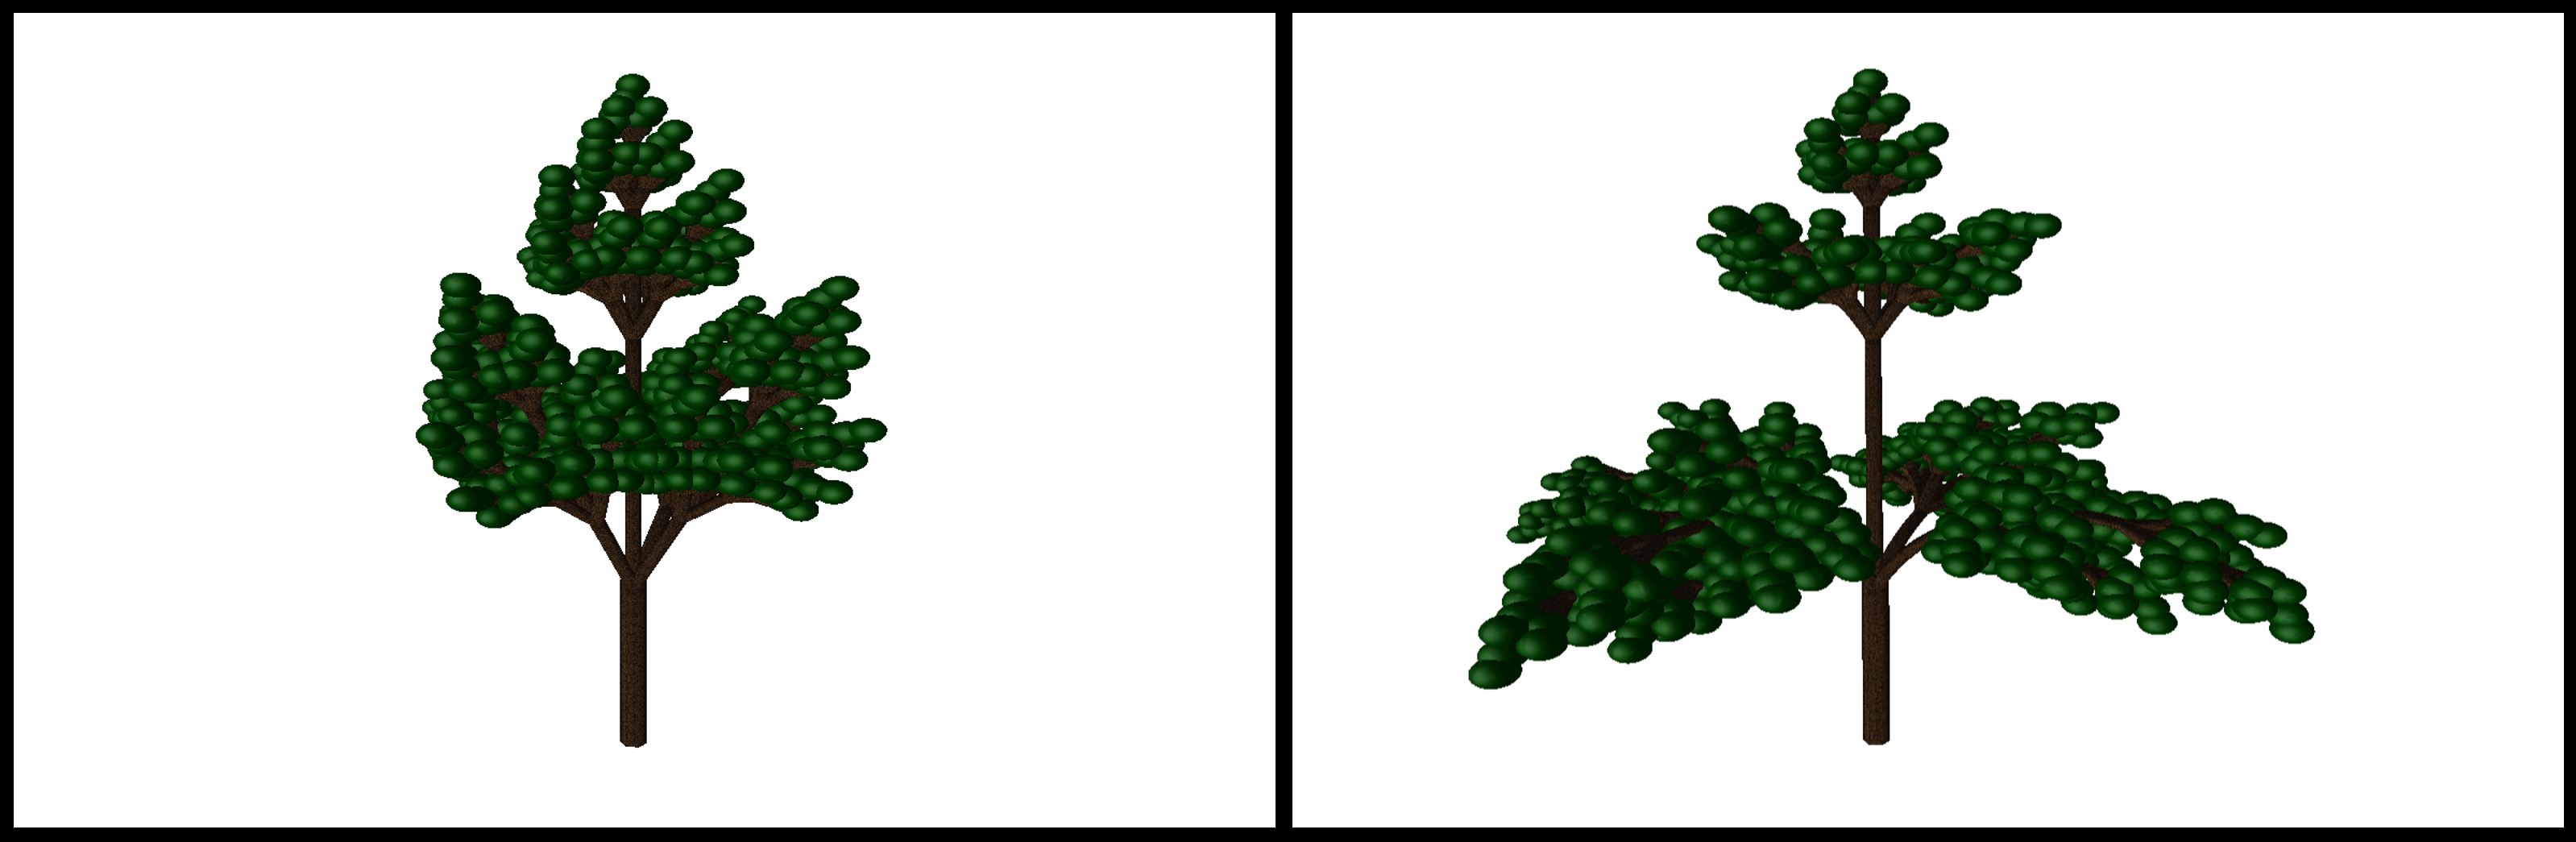
\includegraphics[scale=0.1]{Diagrams/gravityExamples2.png}
		\label{3DAxisFigure} \label{Gravity applied to generated models 2}
		\caption{Simulating gravity on a simple pine tree model.}
	}
\end{figure}
\FloatBarrier

\begin{figure}[htbp]
	{\centering
		\vspace{7px}
		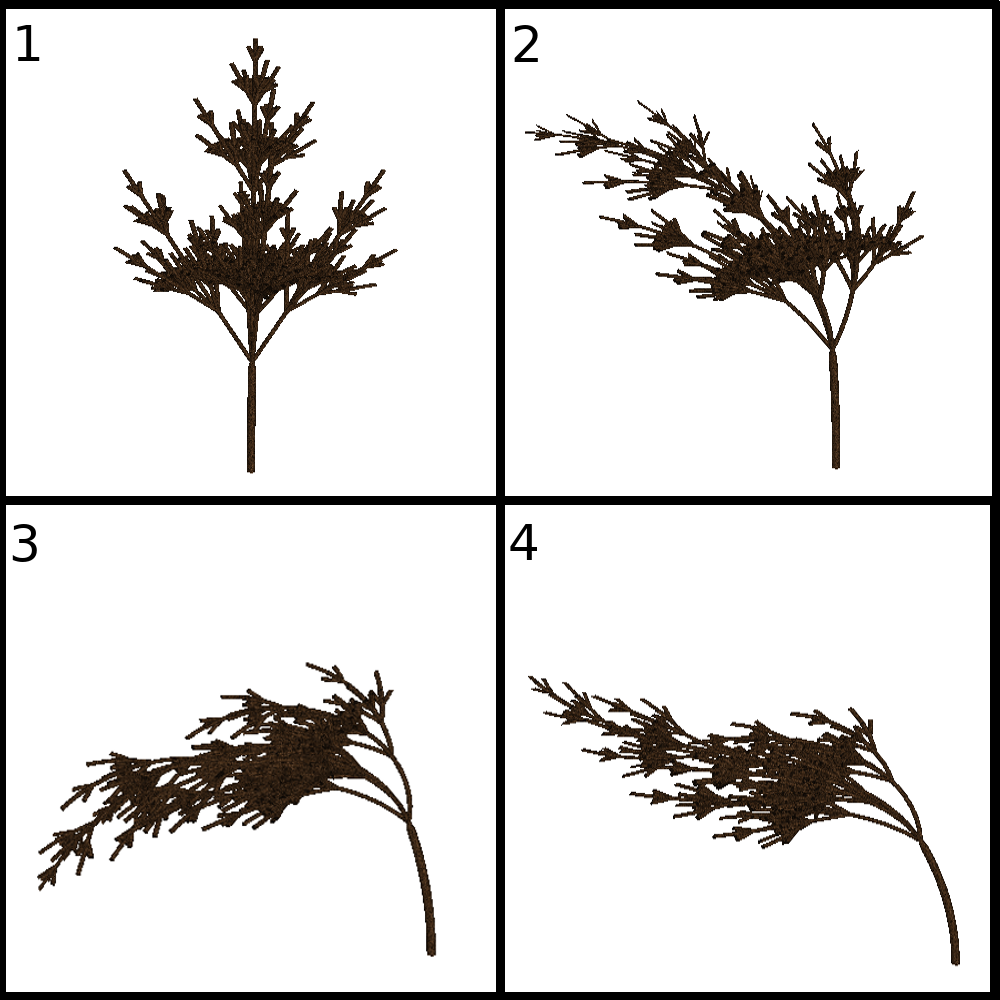
\includegraphics[scale=0.3]{Diagrams/windExample.png}
		\label{3DAxisFigure} \label{Gravity applied to generated models 2}
		\caption{Simulating wind on a simple pine tree model}
	}
\end{figure}
\FloatBarrier


